\RequirePackage[l2tabu,orthodox]{nag}

\documentclass[a4paper,11pt,oneside]{book}

\PassOptionsToPackage{table,svgnames,dvipsnames}{xcolor}

\usepackage[utf8]{inputenc}
\usepackage[T1]{fontenc}
\usepackage[sc]{mathpazo}
\usepackage[american]{babel}
\usepackage[autostyle]{csquotes}
\usepackage[%
  backend=biber,
  url=false,
  style=alphabetic,
  maxnames=4,
  minnames=3,
  maxbibnames=99,
  firstinits,
  uniquename=init]{biblatex} % TODO: adapt bibliography style
\usepackage{graphicx}
\usepackage{scrhack} % necessary for listings package
\usepackage{listings}
\usepackage{lstautogobble}
\usepackage{tikz}
\usepackage{pgfplots}
\usepackage{pgfplotstable}
\usepackage{booktabs}
\usepackage[final]{microtype}
\usepackage{caption}
\usepackage[hidelinks]{hyperref} % hidelinks removes colored boxes around references and links
\usepackage[toc,nonumberlist,acronym]{glossaries} % TODO: remove if glossary not needed
%\usepackage{showframe}


\bibliography{bibliography/literature}


%scrbook
%%%%\setkomafont{disposition}{\normalfont\bfseries} % use serif font for headings
\linespread{1.3} % adjust line spread for mathpazo font

% Settings for glossaries TODO: remove the following block if glossary not needed
\renewcommand{\glsnamefont}[1]{\normalfont\bfseries #1} % use serif font for glossary entry titles
\makeglossaries{}

% Settings for pgfplots
\pgfplotsset{compat=1.9} % TODO: adjust to your installed version
\pgfplotsset{
  % For available color names, see http://www.latextemplates.com/svgnames-colors
  cycle list={CornflowerBlue\\Dandelion\\ForestGreen\\BrickRed\\},
}

% Settings for lstlistings
\lstset{%
  basicstyle=\ttfamily,
  columns=fullflexible,
  autogobble,
  keywordstyle=\bfseries\color{MediumBlue},
  stringstyle=\color{DarkGreen}
}

% Basic information for cover & title page
\newcommand*{\getUniversity}{Technische Universität München}
\newcommand*{\getFaculty}{Department of Informatics}
\newcommand*{\getTitle}{Research and Analysis of Copy Protection Mechanisms for Android Apps, as well as implementing a Sample Application}
\newcommand*{\getTitleGer}{Erforschung und Analyse von Kopierschutzverfahren für Android Apps, sowie Umsetzung in einer Beispielapplikation}
\newcommand*{\getAuthor}{Sebastian Schleemilch}
\newcommand*{\getDoctype}{Master's Thesis in Automotive Software Engineering}
\newcommand*{\getSupervisor}{Prof. Dr. Uwe Baumgarten}
\newcommand*{\getAdvisor}{Nils Kannengießer, M.Sc. }
\newcommand*{\getSubmissionDate}{15.04.2016}
\newcommand*{\getSubmissionLocation}{Munich}
\newcommand*{\Appendixautorefname}{Appendix}
\renewcommand{\texttt}[1]{%
  \begingroup
  \ttfamily
  \begingroup\lccode`~=`/\lowercase{\endgroup\def~}{/\discretionary{}{}{}}%
  \begingroup\lccode`~=`[\lowercase{\endgroup\def~}{[\discretionary{}{}{}}%
  \begingroup\lccode`~=`.\lowercase{\endgroup\def~}{.\discretionary{}{}{}}%
  \catcode`/=\active\catcode`[=\active\catcode`.=\active
  \scantokens{#1\noexpand}%
  \endgroup
}
\newcommand{\code}[1]{\texttt{#1}}

% TODO: add custom commands etc.


%\newglossaryentry{computer}
{
  name=computer,
  description={is a machine that\ldots}
}

\newacronym{app}{App}{Short term for (mobile) installable application}
\newacronym{gui}{GUI}{Graphical User Interface}
\newacronym{hal}{HAL}{Hardware Abstraction Layer}
\newacronym{jni}{JNI}{Java Native Interface}
\newacronym{dvm}{DVM}{Dalvik Virtual Machine}
\newacronym{glibc}{GLIBC}{GNU C Library}
\newacronym{art}{ART}{Android Runtime}
\newacronym{api}{API}{Application Interface}
\newacronym{jvm}{JVM}{Java Virtual Machine}
\newacronym{vm}{VM}{Virtual Machine}
\newacronym{dex}{DEX}{Dalvik Executable}
\newacronym{jit}{JIT}{Just-In-Time}
\newacronym{aot}{AOT}{Ahead-Of-Time}
\newacronym{ndk}{NDK}{Native Development Kit}
\newacronym{jar}{JAR}{Java Library}
\newacronym{apk}{APK}{Android Application Package}
\newacronym{os}{OS}{Operating System}
\newacronym{adb}{ADB}{Android Debug Bridge}
\newacronym{zip}{ZIP}{Zipper file format}
\newacronym{ui}{UI}{User Interface}
\newacronym{ipc}{IPC}{Inter Process Communication}
\newacronym{cpu}{CPU}{Central Processing Unit}
\newacronym{jdk}{JDK}{Java Development Kit}
\newacronym{pm}{pm}{Package Manager}
\newacronym{odex}{ODEX}{Optimized Dalvik Executable}
\newacronym{elf}{ELF}{Executable Linking Format}
\newacronym{uid}{UID}{User Identification Number}
\newacronym{gid}{GID}{Group Identification Number}
\newacronym{oop}{OOP}{Object Oriented Programming}
\newacronym{mime}{MIME}{Internet Media Type}
\newacronym{tis}{TIS}{Tool Interface Standards}
\newacronym{ide}{IDE}{Integrated Development Environment}
\newacronym{pid}{PID}{Process ID}
\newacronym{ppid}{PPID}{Parent Process ID}
\newacronym{aosp}{AOSP}{Android Open Source Project}



\begin{document}

\begin{titlepage}
  % HACK for two-sided documents: ignore binding correction for cover page.
  % Adapted from Markus Kohm's KOMA-Script titlepage=firstiscover handling.
  % See http://mirrors.ctan.org/macros/latex/contrib/koma-script/scrkernel-title.dtx,
  % \maketitle macro.
  \oddsidemargin=\evensidemargin\relax
  \textwidth=\dimexpr\paperwidth-2\evensidemargin-2in\relax
  \hsize=\textwidth\relax

  \centering

  \vspace{0mm}
  
\includegraphics[width=40mm]{logos/tum}

  \vspace{10mm}
  {\huge\MakeUppercase{\getFaculty{}}}\\
  %\vspace{5mm}
  {\large\MakeUppercase{\getUniversity{}}}\\

  \vspace{40mm}
  {\Large \getDoctype{}}

  \vspace{30mm}
  {\huge\bfseries \getTitle{}}

  \vspace{30mm}
  {\LARGE \getAuthor{}}

  \vspace{30mm}
  
\includegraphics[width=20mm]{logos/faculty}
\end{titlepage}


\frontmatter{}
\begin{titlepage}
  \centering

  \vspace{40mm}
  
\includegraphics[width=40mm]{logos/tumBlue}

  \vspace{10mm}
  {\huge\MakeUppercase{\getFaculty{}}}\\

  %\vspace{5mm}
  {\large\MakeUppercase{\getUniversity{}}}\\

  \vspace{20mm}
  {\Large \getDoctype{}}

  \vspace{15mm}
  {\huge\bfseries \getTitle{}}

  \vspace{15mm}
  {\huge\bfseries \getTitleGer{}}

  \vspace{20mm}
  \begin{tabular}{l l}
    Author: & \getAuthor{} \\
    Supervisor: & \getSupervisor{} \\
    Advisor: & \getAdvisor{} \\
    Submission Date: & \getSubmissionDate{} \\
  \end{tabular}

  \vspace{20mm}
  
\includegraphics[width=20mm]{logos/facultyBlue}
\end{titlepage}

\thispagestyle{plain}
\vspace*{0.8\textheight}
\noindent
I confirm that this master's thesis is my own work and I have documented all sources and material used.

\vspace{20mm}
\noindent
\getSubmissionLocation{}, \getSubmissionDate{} \hspace{5cm} \getAuthor{}


%\addcontentsline{toc}{chapter}{Acknowledgments}
\thispagestyle{empty}

\vspace*{2cm}

\begin{center}
{\usekomafont{section} Acknowledgments}
\end{center}

\vspace{1cm}

%TODO: Acknowledgments

\cleardoublepage{}

\chapter{\abstractname}




\microtypesetup{protrusion=false}
\tableofcontents{}
\microtypesetup{protrusion=true}

\printglossaries{}


\mainmatter{}
\pagestyle{fancy}
\fancyhead{}
\fancyhead[C]{\slshape \leftmark}
\fancyfoot[C]{\thepage}

\chapter{Android Status Quo}\label{chapter:android_status_quo}

\section{Popularity of Android}
Android is an operating system by Google,
designed for mobile devices. Version 1.0 was released
in 2008. With a remarkable market share of 82.8\%
it has grown into the most important mobile operating system
followed by Apple's iOS with 13.9\% and Microsoft's Windows
Phone with 2.6\%. See \parencite{Idc15} for a full list
of mobile operating system market shares. While the smartphone
market is still growing, Android did also attach to new
rising platforms like wearables, TV's, cars and general
embedded devices.




\chapter{Android Basics}\label{chapter:android_basics}

\section{Android Architecture}
To provide copy protection mechanisms for Android apps,
of course a deep understanding of the Android system itself
is necessary. As mentioned in~\autoref{chapter:android_status_quo},
Android is built on the Linux kernel. Android does provide not
only shell binaries (Linux kernel) but also a GUI environment
as well as predefined frameworks and a complete environment
for developers to write apps in the Java programming language.
That's why Android is considered to be a ``full software stack''
~\parencite{levin}. Although it's built on Linux,
Google did modify the Linux kernel to their need.
As a result, the Android kernel differs
incompatibly with the Linux kernel since version 2.6.27.

The difference at kernel-level is not massive compared to
the differences at user-mode where Android does have entirely new
components, namely:

\begin{itemize}
\item Dalvik Runtime including the Dalvik Virtual Machine (DVM)
respectively the Android Runtime (ART) since Android version > 5.0.
\item The Bionic C-Library instead of the GNU C Library (GlibC)
\item Hardware Abstraction Layer (HAL)
\item Java Native Interface (JNI)
\item Android specific frameworks
\end{itemize}

\autoref{fig:androidvslinux} visually summarizes the difference
between Android and Linux.

\begin{figure}[htb]
  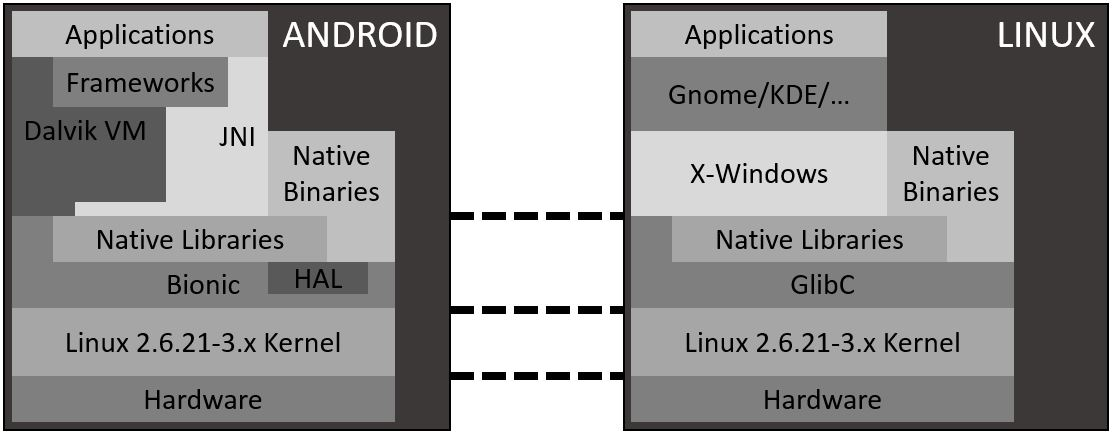
\includegraphics[width=\textwidth]{figures/androidvslinux}
  \caption[Android vs Linux]{Android and Linux comparison
  ~\parencite{levin}}
  \label{fig:androidvslinux}
\end{figure}

The Android specific frameworks are the core work that makes Android
special. They simplify the creation process of applications massively.
Developers can use the high level language Java rather than developing
in C/C++. Additionally, there is a rich set of APIs to solve most of
programmers everyday problems.

In order to get Java programs run on Android, the DVM is introduced
which is quite similar to a Java Virtual Machine (JVM).
The DVM provides an interface between the operating system and
the Java application world, after all the execution of Java programs.
The difference between DVM and JVM is the alternative form of bytecode
which gets executed in the VM. DVM is optimized for mobile devices
in terms of efficiency and sharing memory and is using the
Dalvik Executable format (DEX) as bytecode which is still device
independent ~\parencite{levin}.

With Android version 5.0, Google did introduce ART.
The prior Dalvik runtime does use Just-In-Time (JIT) compiling
where executable machine code is created not until runtime.
ART on the other hand does use Ahead-Of-Time (AOT) compilation
which compiles an app to machine code at installation time.
The reason for JIT in the first place were among other things
storage limitations of mobile devices at the time Android was released
~\parencite{levin}. As a result, the ART apps installation time
is increased as well as the required storage space as a tradeoff
to the app startup and runtime performance. As we will see,
Dalvik is still very much deep-seated in Android even under ART.

The JNI provides an opportunity to write Java programs with embedded
native processor specific code to escape from the VM world
such as direct hardware access.
It is mostly used to optimize the performance for apps (e.g games)
or to hinder reverse engineering of the application code.
Google does provide an Native Development Kit (NDK) to help
developers creating native libraries ~\parencite{ndk}.

Bionic is the Android corresponding GlibC library which was created
for license and simplicity reasons. Overall, it is more lightweight
than the GlibC and well adapted for Android.

Since Android is like to run on a great variety of devices,
it has to support a great amount of different hardware.
The HAL standardizes the interface and allows hardware vendors
to implement their own drivers ~\parencite{levin}.

\section{Android Apps}

\chapter{Copy Protection Status Quo}
\label{chapter:copy_protection_status_quo}

Like introduced in \autoref{chapter:android_status_quo} there
are different goals of copy protection mechanisms starting from
preventing reverse code engineering to protect intellectual property
and reaching to hinder patching to get prohibited access.
The common denominator of those goals is the protection of
the DEX file of every app. A variety of tools do exist that
are able to transform DEX into different readable formats,
modify it and repack it again since the DEX contains
a lot of meta data for its contents (classes, methods, \ldots)
\parencite{dex}.


\section{DEX Dissassembly and Repackaging}
Generally there do exist two possible outcomes of DEX disassembling
- Java code (\code{*.java}) and Smali code (\code{*.smali}).
Since the DEX format is more or less just a different mapping of a
JAR and its containing \code{.class} files, the transition to JAR
is quite simple \parencite{dvminternals}. A tool that is able to
perform this step is ``dex2jar'' \parencite{dex2jartool}.
Along with this JAR, standard Java decompiler like ``JD-GUI''
\parencite{jdtool} can be used to produce the \code{*.java} source code.
If the \code{*.java} is supposed to change and repacked, it can
be again compiled into JAR with Oracle's ``javac'' \parencite{javactool}
followed by Googles ``dx'' tool \parencite{dxtool}
to produce the manipulated DEX.

The alternative way is the use of ``smali/baksmali'' tool
\parencite{smalitool} which is a direct assembler and disassembler
for DEX files rather than taking the Java code detour. There is also
a tool included that can convert the ODEX back to DEX.

Overall, the dissassembly of unchanged DEX is quite easy and is shown
as a concluding overview in \autoref{fig:dex_disassembly}

Therefore several countermeasures were established which are
described in the following sections.

\begin{figure}[htb]
  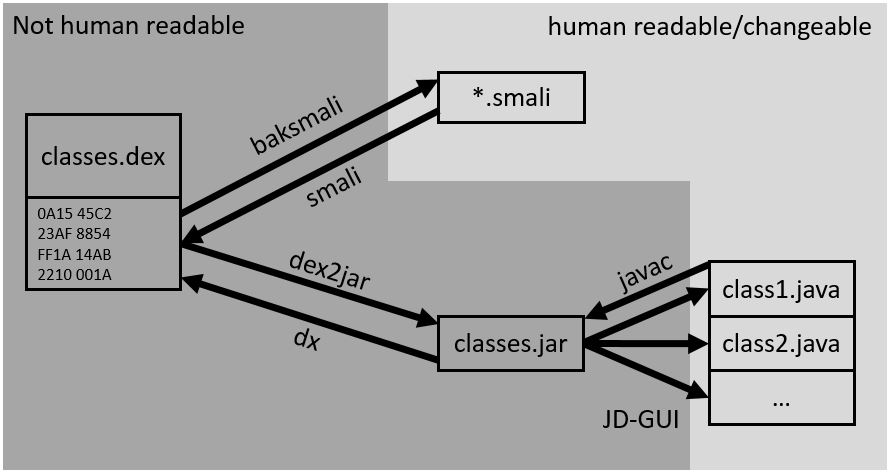
\includegraphics[width=\textwidth]{figures/dex_disassembly}
  \caption[DEX Assembly/Disassembly]{DEX Assembly/Disassembly}
  \label{fig:dex_disassembly}
\end{figure}


\section{Obfuscation Techniques}
Obfuscation in the context of copy protection for application
is generally the term for hardening an application against
reverse code engineering techniques. It can be achieved by different methods
that can be seperated in two main groups, static and dynamic obfuscation.
Static means that the obfuscation technique is applied to code units (source
code, binaries, ...) while the application is not executed. Therefore an
attacker could possibly successful analyze the application without executing it
if he manages to break this obfuscation. Applications that are dynamically
obfuscated on the other hand, are much harder to analyze since the behavior
of the application is not decided until its execution. An attacker needs to connect to the process of the application followed by a just in time inspection.

It does follow a list of common static and dynamic obfuscation techniques
for Android applications.

\subsection{Static}
\subsubsection{Common Source Code Obfuscation}
The most common way of harden source code is to remove any kind of meta data
that has been added during the development process. Means destroying/modifying
information that originally was present in the source code.
This technique can be applied at different layers, \code{.java}, \code{.class} and the final \code{.dex} in case of Android.
Among other things they consist of renaming
classes, variables, functions, irreducable code insertion,
artificial parallelization, method inlining/outlining, unrolling
loops, encoding strings, changing the control flowand so on to confuse code analysts but always keeping its original behavior.

Popular tools for that purpose are Google's ``ProGuard''
\parencite{proguardtool} which is included in the Android build system and
can be enabled easily as well as``DexGuard'' by GuardSquare
\parencite{dexguardtool}. ``ProGuard'' does
operate on source code level where ``DexGuard'' operates on DEX.
Since the first unit of Android applications is Java code, classical Java
obfuscators also can be used.

\subsubsection{Junk-Byte-Insertion}
Junk-Byte-Insertion's goal is to confuse static analyzing
disassembling tools. It does work for tools with the
``linear sweep'' method to analyze a file. That means
the tools are processing every instruction from the entrypoint
till the end without interpreting them (e.g. not following jumps).
That examining technique can be exploited to break the disassembling
procedure. Let's assume we do have the code snippet of
\autoref{fig:junk_byte_listening}
on source code level.

\begin{figure}[htb]
  \centering
  \begin{tabular}{c}
  \begin{lstlisting}[language=Java]
    if (false) {
        0x12 0x34 0x56
    } else {
        proceedProgram()
    }
  \end{lstlisting}
  \end{tabular}
  \caption[Junk-Byte-Insertion]{Junk-Byte-Insertion Example}
  \label{fig:junk_byte_listening}
\end{figure}

Cause of the if-condition, the \code{insertBreakingBytes()} method is never
reached. Since ``linear sweep'' does not perform jumps, the analyzing tool
is trying to revert those bytes into source code. By choosing a specific
sequence of bytes, the transformation will fail.

Enhanced tools will use the ``recursive traversal'' technique to analyze a
file which is capable of detecting dead branches like in the example above.
These tools also may be tricked by choosing a more complicated condition for
if-conditions that can only be evaluated at runtime and therefore the
whole conditional branch (including the breaking byte sequence) would also be evaluated.
\parencite{lvl_imp}.

\subsection{Dynamic}
\subsubsection{Hidden Methods Invocation}
\subsubsection{Dynamic Code Loading}
\subsubsection{Self Modifying Code}


\chapter{ART Internals: App Executable Format}
\label{chapter:art_internals_app_executable_format}

A core element of the recently introduced ART is the file that
gets created by ``dex2oat'' during the installation time of an app,
described in \autoref{section:app_installation}.
Since ART does use AOT compilation, the file format is expected
to be an executable or at least a native code container.
A lot of copy protection mechanisms are based on the use of native
code because it is supposed to be more secure from reverse code
engineering (which is an assumption so far).
Therefore it's worth to have closer look at that file format
especially since Google does not provide any further information
about it's content and it might have the potential of
revolutionizing the available copy protection mechanisms for
Android or having at least a great impact on them.

By applying the Unix command ``\code{file}'' (which can classify
files to MIME-types) to the resulting file of the ``\code{dex2oat}''
tool it comes apparent that it's a particular ELF file (32 or 64 bit)
called OAT file from now on.

\section{ELF File Format}\label{section:elf_file_format}
ELF originally was originally specified by UNIX System Laboratories
(USL) and later by Tool Interface Standards (TIS) and is a common
standard for executables, object code and shared libraries on UNIX
systems. It's a quite flexible format for different CPUs and
architectures and does serve as a container for different
executable binary formats.

\begin{figure}[htb]
  \centering
  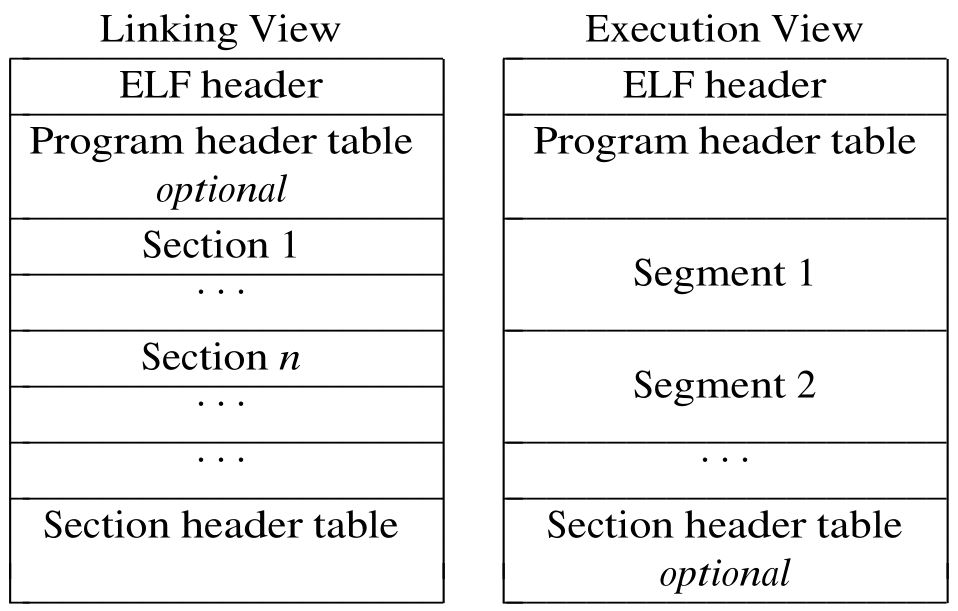
\includegraphics[scale=0.4]{figures/elf_format}
  \caption[ELF file format]{ELF file format taken from \parencite{portable_formats_spec}}
  \label{fig:elf_format}
\end{figure}

The \autoref{fig:elf_format} shows the file structure.
One have to differentiate the context of how the file is viewed.
While a linker does care about sections, sections may be
glued together to segments when executing the file.
Meta data about the file can be read out of the ``ELF header''
that starts at adress \code{0x00} and does contain
information about the version, file type, target machine and
offsets to the program- and section header tables.
In ART, the file is marked as an shared object with LSB encoding
and not as an executable which makes clear that this file is not
supposed to get executed directly but to be linked first
(An open question remains so far which process is then starting
the app).
Segments are referenced by the program header table and sections
by the section header table. For an execution process, only the header
and the information out of the program header table is needed
\parencite{life_of_binaries}.

Let's first have a look at the used sections in case of the specific
Android implementation, the OAT file:
\autoref{fig:section_headers} does show the output of
``\code{readelf -S <ELF-App-File>}'', listening all available sections

\begin{figure}[htb]
  \centering
  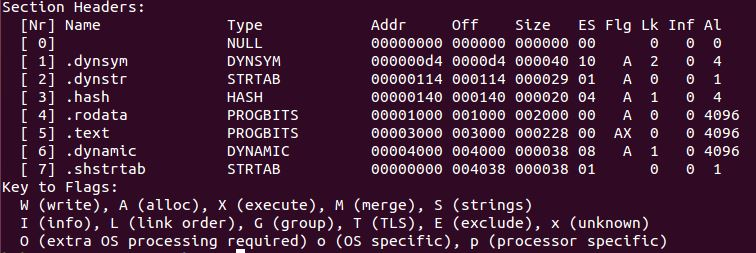
\includegraphics[width=\textwidth]{figures/android_elf_section_headers}
  \caption[ELF section headers]{ELF section headers}
  \label{fig:section_headers}
\end{figure}

It does follow a short description of sections that are implemented
\parencite{life_of_binaries}:
\begin{itemize}
    \item \code{.dynsym} holds a dynamic linking symbol table that
    does contain information for locating and relocating a program's
    symbol definitions and references. It does contain ``oatdata'',
    ``oatexec'' and ``oatlastword'' in case of an OAT file.
    \item \code{.dynstr} does hold strings for dynamic linking,
    mostly names that are referenced by \code{.dynsym}.
    \item \code{.hash} contains the symbol hash table
    \item \code{.rodata} stands for ``Read-Only data'' and does
    contain arbitrary data whose interpretation is solely
    determined by the program itself. We will
    see that in case of Android it does hold the actual OAT file
    that will be further described in \autoref{section:oat_file}.
    \item \code{.text} is the only region that is marked as
    executable and therefore it does hold the main body of
    program code.
    \item \code{.dynamic} includes dynamic linking information.
    \item \code{.shstrtab} stands for ``Section header string
    table'' and therefore contains the previous described
    section names including its own (e.g. ``\code{.shstrtab}'').
\end{itemize}

\autoref{fig:program_headers} shows the alternative view of the
file by having a look at segments (``\code{readelf -S <ELF-App-File>}'')
. Type ``PHDR'' stands for ``Program header''. Segments with type
``LOAD'' are supposed to be loaded from disk into memory while
a ``DYNAMIC'' segment is a part of a ``LOAD'' segment and is equal
to the ``\code{.dynamic}'' section. The mapping of ``LOAD'' segments
into memory is performed by respecting the alignment of \code{0x1000}
means that only chunks of that size (or a multiple) are being read
(e.g. reading the segment at \code{0x3000} will copy the content
from \code{0x3000-0x4000} even if the size only equals \code{0x340}).
The difference between ``FileSiz'' that obviously stands for the file
size and ``MemSiz'' that stands for memory size is the space that
gets reserved for uninitialized variables.
\begin{figure}[htb]
  \centering
  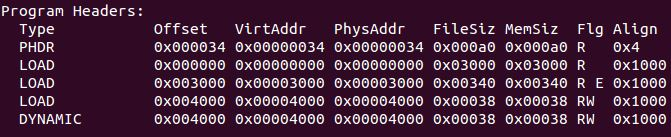
\includegraphics[width=\textwidth]{figures/android_elf_program_headers}
  \caption[ELF program headers]{ELF program headers}
  \label{fig:program_headers}
\end{figure}
The \code{readelf} tool is also capable of showing the resulting
mapping of sections to segments
(\autoref{fig:sections_segments_mapping}).

\begin{figure}[htb]
  \centering
  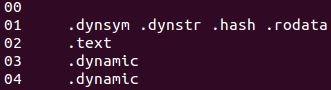
\includegraphics[scale=0.7]{figures/section_segment_mapping}
  \caption[ELF section segment mapping]{ELF section segment mapping}
  \label{fig:sections_segments_mapping}
\end{figure}

It's interesting to note that the Android usage of ELF for apps
is very minimalistic and does contain very few sections/segments
compared to a common program written in C/C++ (\code{helloWorld.c}
does include over 30 sections). As described before,
\code{.dynsym} does contain entries which tell us where to find
the OAT data, specifically the ``oatdata''(equals \code{.rodata})
and the ``oatexec'' (equals \code{.text})
section that will now be analyzed.

\section{OAT File}\label{section:oat_file}
Google does not provide any official documentation about the OAT
file format other than the source code itself
(\code{art/runtime/oat[\_file].h[c]}). \parencite{hiding_behind_art}
however gives a helpful introduction and an overview is given
in \autoref{fig:oat_format} that shows the content of ``oatdata''.

\begin{figure}[htb]
  \centering
  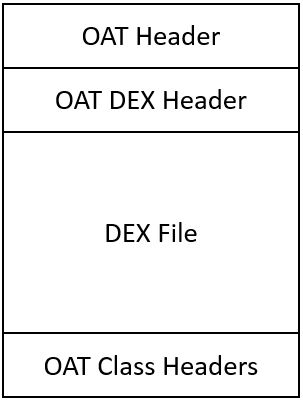
\includegraphics[scale=0.5]{figures/oat_format}
  \caption[OAT format]{OAT format}
  \label{fig:oat_format}
\end{figure}

Important attributes that the ``OAT Header'' contains are the
checksum over itself,
the instruction set (ARM, ARM64, MIPS, \ldots), the executable
offset from start of ``oatdata'' and the quantity of embedded
DEX files (that should be one and does exist for flexibility
reasons). It does follow the ``OAT Dex Header'', containing
the absolute path of the original DEX file, the checksum, the
offset to the copy of the DEX file that is embedded as well as
an offset to the ``OAT Class Headers''. ``OAT Class Headers''
do offer information about defined classes. First, the type
of class which contains how many methods in the class
are compiled to native code (``all'', ``some'' or ``none'' but
should be ``all'' in almost every case) and secondly
the offsets to the native code begin of every compiled method.
The actual code is located in a superordinated section
(\code{.text}) which is seperated but referenced from this one.

\section{DEX File Format}
\label{section:dex_file_format}
To be complete, we will also have a quick look into the DEX format,
which is officially documented by Google \parencite{dex}.
Before the introduction of ART, DEX was the last unit before
execution of an app (besides ODEX). However, the DVM does accept
both formats thats why it is possible to dynamically execute
DEX without the transformation step. DEX does not only contain
the VM instructions but some meta data to locate
higher abstaction level information like classes and within that
methods, fields, \ldots.

\autoref{fig:dex_format} does show the file layout.
\begin{figure}[htb]
  \centering
  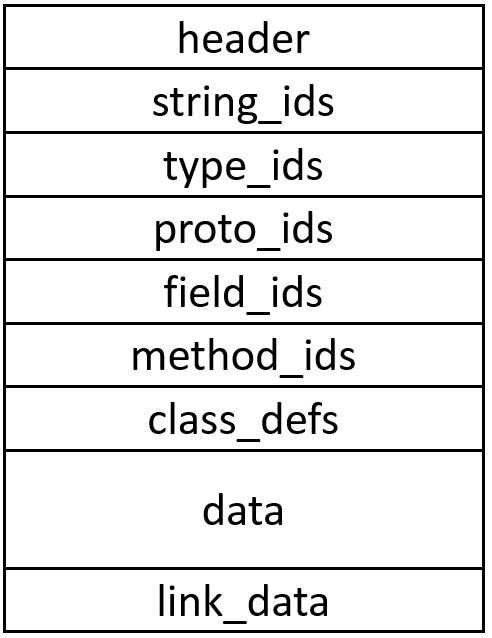
\includegraphics[scale=0.3]{figures/dex_format}
  \caption[DEX format]{DEX format}
  \label{fig:dex_format}
\end{figure}
The header again includes a checksum of the whole file (checksum
field excluded), the overall size as well as the offsets and sizes
of every section. Sections with ``ids'' ending are arrays of
id items of their type and do reference
a data item in the ``data'' section or are specifying
an index into another ``ids'' section. A ``string\_id'' item for
instance does just contain an offset from file beginning
that should be located in ``data'' whereas the ``type\_id'' item
includes an index into the ``string\_ids'' field. The principle
of the file structure is therefore a nesting architecture of
sections. The ``class\_def'' section does contain methods that
in turn include strings, fields and so on. Content is being
stored exclusively in the data section. In the end,
executable VM instructions are referenced from methods.


\section{Conclusion}\label{section:andelf_format_conclusion}
The runtime transition from DVM to ART of course had to result
in a new file that gets intepreted/executed when an app starts.
However, the change is not as smooth as expected since
the new file format is not pure executable code but, as
discovered in this chapter, a combination of native code
and embedded DEX code as well as a new OAT file format
which references parts of the native code. Also, there is some
confusion for what part the name ``OAT file'' stands. On the
one hand, Google's documentation files and the naming
convention of the``dex2oat'' tool are giving the impression
that the file as a whole is an ``OAT file''. On
the other hand, the file is a valid implementation of the
well known ELF format and contains a section that starts
with bytes known by MIME types with ``.oat'' as file format
(.rodata section). Additional, the ``oatexec'' section
is controlled via the greater ELF format. Therefore
, ``OAT file'' stands most likely for both of those meanings, the
Android app specific and minimalistic implementation of the ELF
as well as the combination of the ``oatdata'' and ``oatexec''
section to a file alike entity. \autoref{fig:andelf_format} does
provide an overall view of the fileformat of ART app executables.

\begin{figure}[htb]
  \centering
  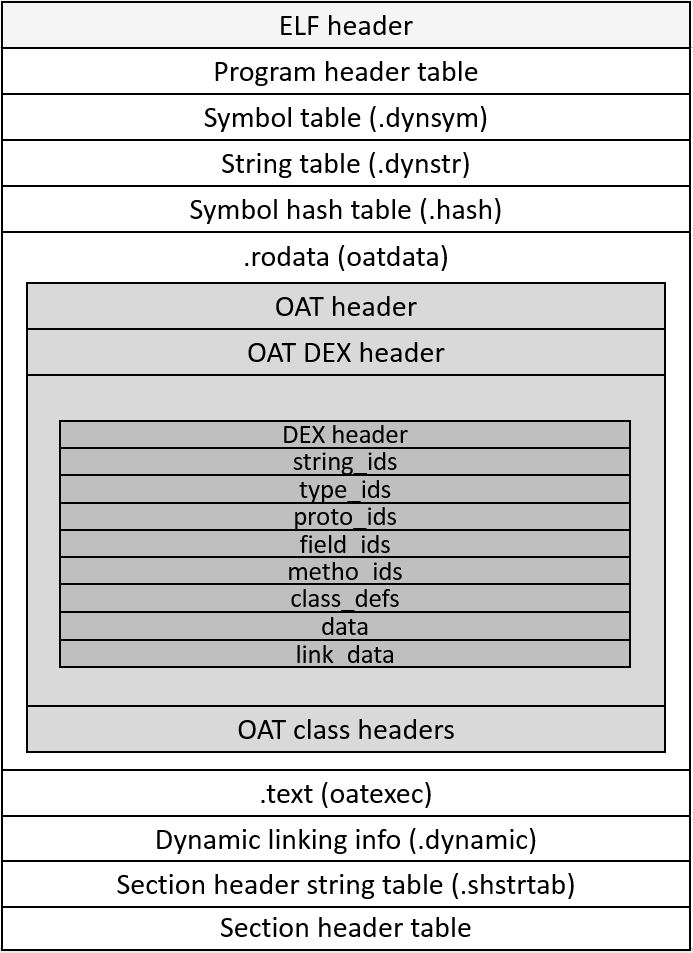
\includegraphics[scale=0.5]{figures/andelf_format}
  \caption[ART app executable format]{ART app executable format}
  \label{fig:andelf_format}
\end{figure}

The awareness of the detailed executable file format does pop
new questions about the ART Android internals.
Since the file is marked as an shared object, it won't get
executed as a standalone program but most likely will be also
included in a forked Zygote process like in the Dalvik runtime.
However it is not clear which parts of the OAT file are
needed to run an app adequately. Is the embedded DEX for instance
mandatory for the app to work correctly? As we have seen in
\autoref{chapter:copy_protection_status_quo}, DEX files are
a crucial part of applications to protect. What if that part
can be missed out by distributing a minimal stub application
followed by a dynamic native code injection at runtime?
It is also interesting if and how the known dynamic obfuscation
techniques, described in \autoref{section:obfuscation_techniques},
can be applied to ART apps since there is no VM bytecode that can
be manipulated at runtime but only native code.
Therefore a deep understanding for the app init and execution
process under ART is a precondition to answer these
questions and has to be way more detailed than described in
\autoref{section:app_execution}.

\chapter{ART Internals: App Execution}
\label{chapter:art_internals_app_execution}

A running app can be tracked with linux tools that are capable
of showing processes like ``\code{ps}''. To investigate the app execution
we therefore have to open a root shell at the target device
(device should be rooted) with ``\code{adb shell}''
followed by an ``\code{su}'' command after getting the
device prompt (``\code{shell@flounder:/ \$}''). It will then change
to ``\code{root@flounder:/ \#}''. A ``\code{ps}'' command will display
useful information like it's ``USER'', the process id ``PID'',
the process id of its parent ``PPID'' and of course the actual name.
Interesting entries for further inspection are being displayed in
\autoref{tab:ps_entries}.

\begin{table}[htb]
  \caption[Android processes]{Android processes}
  \label{tab:ps_entries}
  \centering
  \begin{tabular}{l l l l l}
    \toprule
      USER & PID & PPID & ... & NAME \\
    \midrule
      root & 1 & 0 & ... & /init \\
      root & 211 & 1 & ... & zygote64 \\
      root & 212 & 1 & ... & zygote \\
      u0\_a137 & 10072 & 211 & ... & ma.schleemilch.helloandroid \\
      u0\_a35 & 11017 & 212 & ... & com.android.chrome \\
    \bottomrule
  \end{tabular}
\end{table}

The process ``\code{/init}'' is the first process of Android (although
it has a parent with PID ``0'' which is the process scheduler at kernel
level).
Furthermore, every user and system app has either the process
``\code{zygote}'' or ``\code{zygote64}'' as its parent depending
if the app was written for 32 or 64 bit. That makes clear that apps
are forked from the Zygote process that is in turn forked out of
``\code{/init}''. Even more detailed information about processes can be
pulled out of the ``\code{/proc}'' directory. It is an interface to the
kernel and does contain a folder for every process, named after its PID
\parencite{proc}. The most attractive attribute of that folder is
``\code{exe}'' which is a symbolic link to the executable that started
the process. Since apps are a fork of Zygote, they should point
to the same executable, which they do (see \autoref{tab:process_executables}).

\begin{table}[htb]
  \caption[Process starting executables]{Process starting executables}
  \label{tab:process_executables}
  \centering
  \begin{tabular}{l l}
    \toprule
    \multicolumn{2}{l}{root@flounder:/ \# ls -la /proc/10072/exe} \\
    ... & exe -> /system/bin/app\_process64\_original\\
    \midrule
    \multicolumn{2}{l}{root@flounder:/ \# ls -la /proc/211/exe} \\
    ... & exe -> /system/bin/app\_process64\_original\\
    \midrule
    \multicolumn{2}{l}{root@flounder:/ \# ls -la /proc/11017/exe} \\
    ... & exe -> /system/bin/app\_process32\\
    \midrule
    \multicolumn{2}{l}{root@flounder:/ \# ls -la /proc/212/exe} \\
    ... & exe -> /system/bin/app\_process32\\
    \bottomrule
  \end{tabular}
\end{table}

An executable named ``\code{app\_process32/64}'' seems like to be the entry-point for apps to be started. The responsible program of that executable
can be found in the Android Open Source Project (AOSP) where
``\code{app\_main.cpp}'' is the name of the source code file that gets
compiled into ``\code{app\_process32}'' and ``\code{app\_process64}''
and can be found at ``\code{/frameworks/base/cmds/app\_process/}''.
In the next section, the logic and the content of that program will be analyzed based on the Android 5.1 AOSP version.

\section{Functionality of ``\code{app\_main.cpp}''}
\label{section:app_main}
The best thing to do when analyzing source code is to start at the
``\code{main()}'' method. One of the first things the program does is
creating a new ``\code{AppRuntime runtime}'' object that inherits from the
\code{AndroidRuntime} class but does override a few functions. As parameters it will expect the \code{argv[0]}
which is the program name itself as well as the total length of arguments.
In the end we will see that the program transfers the flow control to this object by calling the \code{runtime.start()} method. As expected, there
are different modes this program can act as, specifying ``\code{-{}-zygote}'',
``\code{-{}-start-system-server}'' and more important ``\code{-{}-application}'' arguments.
If the ``\code{-{}-application}'' argument is present, there will be also following ``\code{className}'' attribute specifying it's main class.
The runtime object gets filled with the given arguments, ready for take
over the control and finally calling the method ``\code{runtime.start("com.android.internal.os.RuntimeInit", args);}'' in case of an application
where ``\code{args}'' does only contain ``application''(see \autoref{rt_start}) and ``\code{args}'' has been initialized just a few lines before. So the information about which app should be started is being determined
when the runtime gets filled with arguments like shown in \autoref{rt_special}

\lstinputlisting[language=C++, caption=Runtime Specialization, label=rt_special,firstline=267, lastline=275]{"code/app_main.cpp"}

\lstinputlisting[language=C++, caption=Runtime Start, label=rt_start,firstline=306, lastline=310]{"code/app_main.cpp"}

As we've seen, a runtime object will be created for every new process and
therefore also for apps. All given arguments to ``\code{app\_process32/64}''
are forwarded to the runtime object and an additional parameter (``application'') describing which form of process will be created and is then being pushed
into the ``\code{runtime.start()}'' method.
After all, the initialized runtime does know that it should start an application with its given main class name. Also the actual process name
has been changed to a ``nice name'' that also has been defined as a command
line parameter. \autoref{fig:app_process} visualizes the argument parsing
of the program.
The obviously next thing to do to get further to the goal of knowing which parts of the OAT file format out of \autoref{chapter:art_internals_app_executable_format} gets executed when starting an app is to have a look at the ``AndroidRuntime'' class implementation.

\begin{figure}[htb]
  \centering
  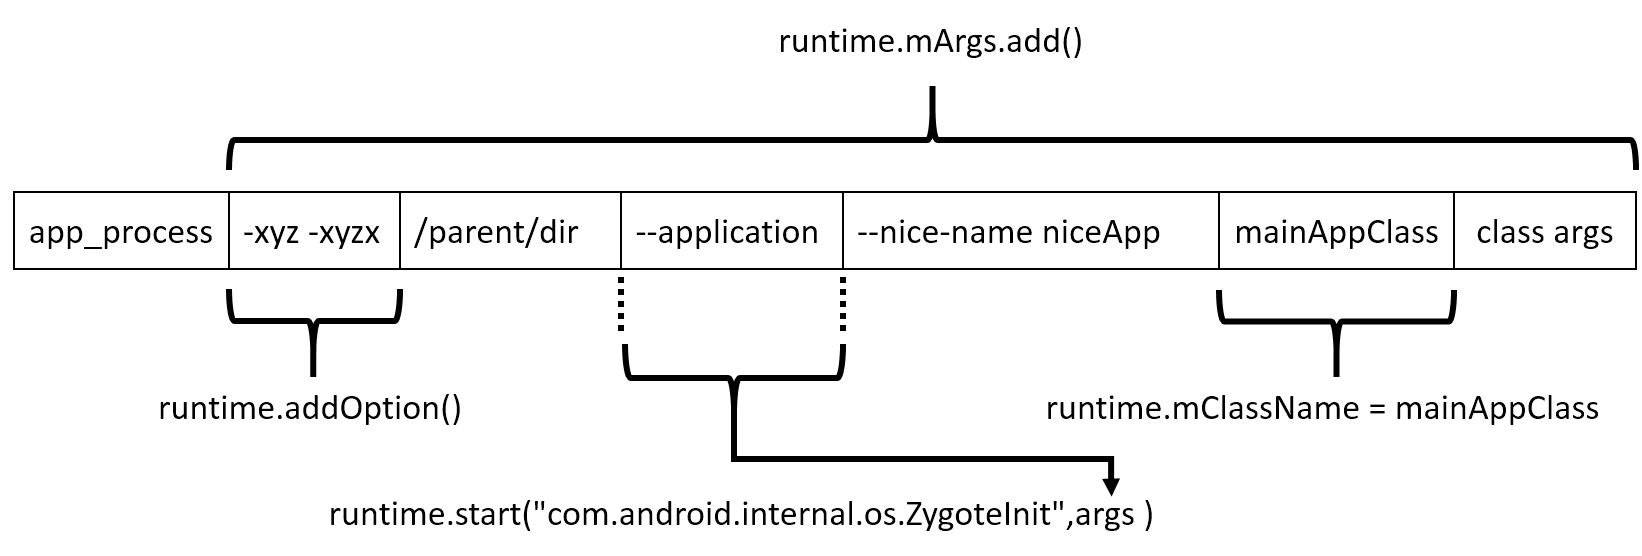
\includegraphics[width=\textwidth]{figures/app_process}
  \caption[App Process Argument Parsing]{App Process Argument Parsing}
  \label{fig:app_process}
\end{figure}


\section{Functionality of ``\code{AndroidRuntime.cpp}''}
The source file can be found at the path ``\code{/frameworks/base/core/jni/AndroidRuntime.cpp}''. As described in \autoref{section:app_main}, first the runtime constructor gets called followed by setting a few options as well as
the class name and all arguments and finally a call of the ``\code{start()}''
method. So a good start should be the constructor. It is quite short and
does reserve some space for options and is initializing a pointer to the object
itself.
The ``\code{start()}'' method does expect a class name (``.../ZygoteInit'') and a vector or args which is only one in this case. It follow
special log events in case of a system server start and a check if the root
dir ``\code{/system}'' does exist in the environment of linux.





\appendix{}
 % TODO: remove if glossary not needed
\glsaddall{} % add all defined terms to glossary, even if not referenced in text
\microtypesetup{protrusion=false}
\listoffigures{}
\listoftables{}
\lstlistoflistings
\microtypesetup{protrusion=true}
\printbibliography{}

\end{document}
